\documentclass[12pt]{article}
\usepackage[brazilian]{babel}
\usepackage[utf8]{inputenc}
\usepackage[T1]{fontenc}
\usepackage{listings}
\usepackage{color}
\usepackage{morefloats}
\usepackage{amsmath}
\usepackage{float}
\usepackage{graphicx}

\restylefloat{table}

\definecolor{dkgreen}{rgb}{0,0.6,0}
\definecolor{gray}{rgb}{0.5,0.5,0.5}
\definecolor{mauve}{rgb}{0.58,0,0.82}

\lstset{frame=tb,
  aboveskip=3mm,
  belowskip=3mm,
  showstringspaces=false,
  columns=flexible,
  basicstyle={\small\ttfamily},
  numbers=none,
  numberstyle=\tiny\color{gray},
  keywordstyle=\color{blue},
  commentstyle=\color{dkgreen},
  stringstyle=\color{mauve},
  breaklines=true,
  breakatwhitespace=true
  tabsize=3
}

\sloppy

\title{Algoritmos e Programação III\\ Trabalho II}

\author{Matthias Oliveira de Nunes}

\begin{document}

\maketitle

\begin{abstract}

Este artigo descreve uma alternativa de solução para o segundo trabalho proposto
pela disciplina de Algoritmos e Programação III, que consiste em descobrir o
maior número de filmes a serem assistidos, um após o outro, a partir de um
arquivo contendo as informações de cada filme. Foram fornecidos seus horários de
início e fim, e o algoritmo trata de achar a maior sequência possível a ser
assistida.

\end{abstract}

\section{Introdução}

Dentro do escopo da disciplina de Algoritmos e Programação III, o segundo
problema pode ser resumido como o seguinte: o clube de cinema de Porto Alegre
quer achar a maior sequência de filmes que podem ser assistidos, um após o
outro, em um domingo. Assim podem otimizar o seu tempo e aproveitar ao máximo.
Para ajuda-los, desenvolveremos um programa que recebe uma lista de filmes e
seus horários de início e fim, e depois determina a maior sequência possível a
ser assistida.

A entrada, possui o formato mostrado a seguir:  A primeira linha informa $k$,
que é o número de filmes existentes. Depois seguem $k$ linhas indicando o
horário de início e de fim de cada cada um, com seus nomes logo em seguida.

\vspace{2.0cm}

\begin{lstlisting}

10
07:30 09:20 Filme_1
07:57 09:40 Filme_2
10:43 12:38 Filme_3
08:59 10:59 Filme_4
09:44 11:36 Filme_5
02:25 04:09 Filme_6
03:21 05:01 Filme_7
10:36 12:07 Filme_8
10:24 12:23 Filme_9
01:07 02:58 Filme_10

\end{lstlisting}

\vspace{0.5cm}

O algoritmo será testado em casos de teste previamente fornecidos, e ao final do
programa, devem ser apresentadas as seguintes informações:

\begin{enumerate}

\item Identificação do caso de teste.

\item Resultado do caso de teste: número de filmes que podem ser assistidos e identificação dos filmes.

\item Tempo de execução do algoritmo.

\end{enumerate}

Junto a isso, foi pedido que fosse fornecido resultado para pelo menos 8 casos
diferentes e não considerar tempo de deslocamento entre filmes, isto é, se um
filme acaba às 10:00 e outro começa nesse mesmo horário, é possível assistir um
e depois o outro.

\section{Algoritmo}

Depois de considerar o problema, a solução que encontramos vai ser desenvolvida
em duas partes: Montar um grafo dirigido, a partir da lista, onde cada nodo
corresponde a um filme, e achar o maior caminho existente nesse grafo. Se cada
nodo representa um filme, seus vizinhos serão todos os filmes que podem ser
assistidos após o mesmo, logo, o maior caminho é a maior sequência de filmes
possível.

\subsection{Montar o grafo}

Para montar o grafo, foi usado um algoritmo muito simples de entender:
Considerando que cada nodo representa um filme, para cada nodo $u$ a ser
adicionado e para cada nodo $v$ já existente no grafo, se o horário de término
de $v$ for antes do horário de início de $u$, adiciona a aresta $v \rightarrow
u$ no grafo, se o horário de início de $v$ for depois do horário de término de
$u$, adiciona a aresta $u \rightarrow v$ no grafo.

O método inserirNodo é chamado para cada nodo que será inserido no grafo, vendo
ele em pseudo-código fica:

\begin{lstlisting}

inserirNodo(Node u) {
    para cada nodo v do grafo {
      se (v.getFim() < u.getInicio())
        InsereAresta(v, u);
      se (v.getInicio() > u.getFim())
        InsereAresta(u, v);
    }
  }

\end{lstlisting}

Não tem como fugir muito desse raciocínio, já que somos obrigados a percorrer os
nodos para descobrir quais que podem se conectar com o novo nodo inserido. Na
implementação real, foi adicionado um teste para validar as informações
fornecidas, por exemplo, o horário de início de um filme não pode ser mais tarde
que o horário de fim.

\subsection{Descobrir a maior sequência}

Para descobrirmos a maior sequência de filmes possível, utilizamos um algoritmo
recursivo cuja idéia é: Vamos perguntar a um nodo qual a maior caminho que
existe a partir dele, ele irá perguntar a mesma coisa para cada um de seus
vizinhos, e quando um nodo não tem vizinhos, ele retorna ele mesmo. Quando um
nodo recebe a resposta dos seus vizinhos, ele retorna o maior de todos os
caminhos retornados se incluindo nesse caminho. A idéia pode ser demonstrada
observando este grafo:

\begin{figure}[H]
\centering
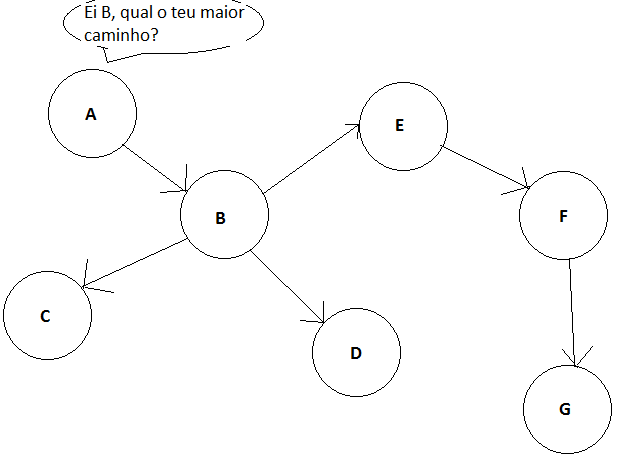
\includegraphics[width=100mm]{graphA.png}
\caption{A perguntando à B}
\label{graphA}
\end{figure}

\begin{figure}[H]
\centering
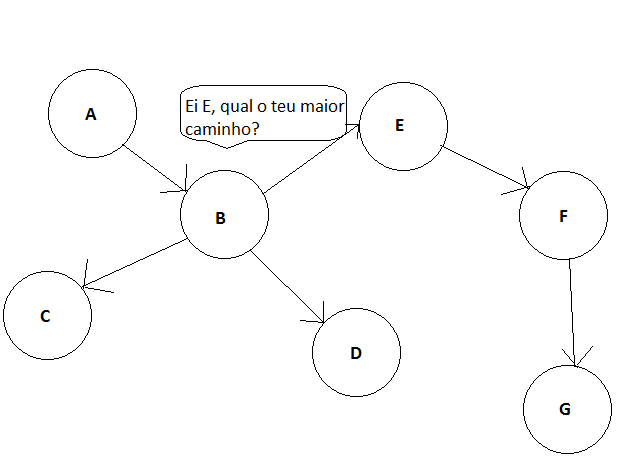
\includegraphics[width=100mm]{graphB.png}
\caption{B perguntando à todos seus vizinhos}
\label{graphB}
\end{figure}

B pergunta isso a todos os seus vizinhos, mas nas figuras só iremos mostrar ele
perguntando ao nodo E.

\begin{figure}[H]
\centering
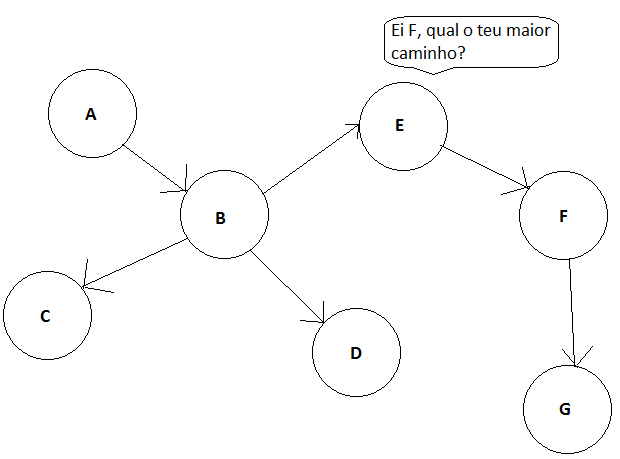
\includegraphics[width=100mm]{graphE.png}
\caption{E perguntando à F}
\label{graphE}
\end{figure}

\begin{figure}[H]
\centering
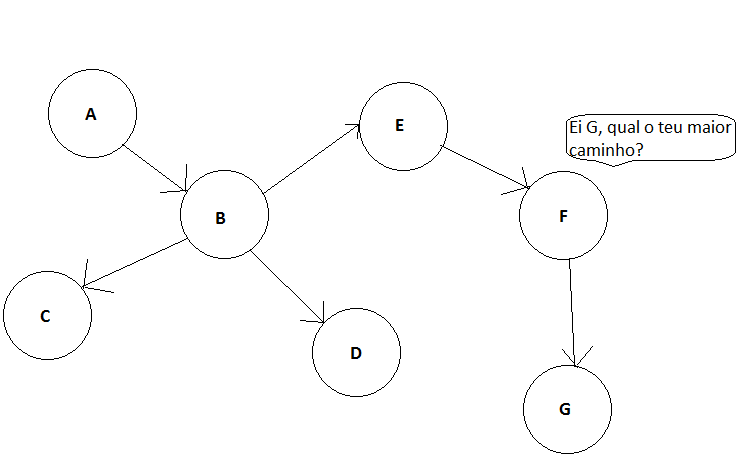
\includegraphics[width=100mm]{graphF.png}
\caption{F perguntando à G}
\label{graphF}
\end{figure}

\begin{figure}[H]
\centering
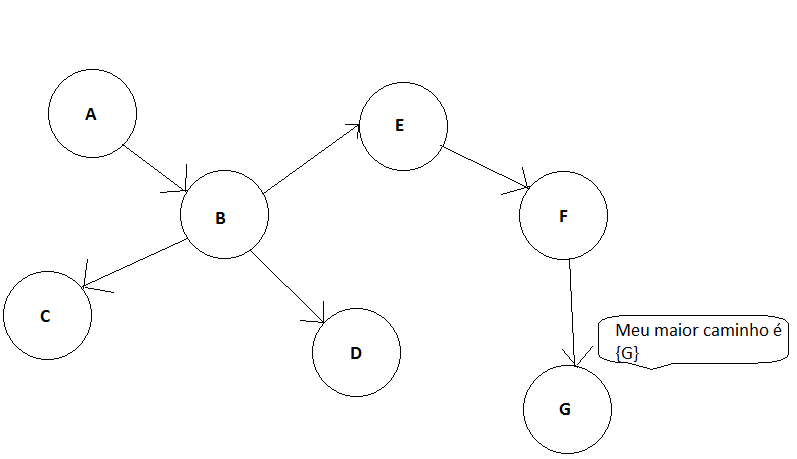
\includegraphics[width=100mm]{graphGr.png}
\caption{G respondendo à F}
\label{graphGr}
\end{figure}

\begin{figure}[H]
\centering
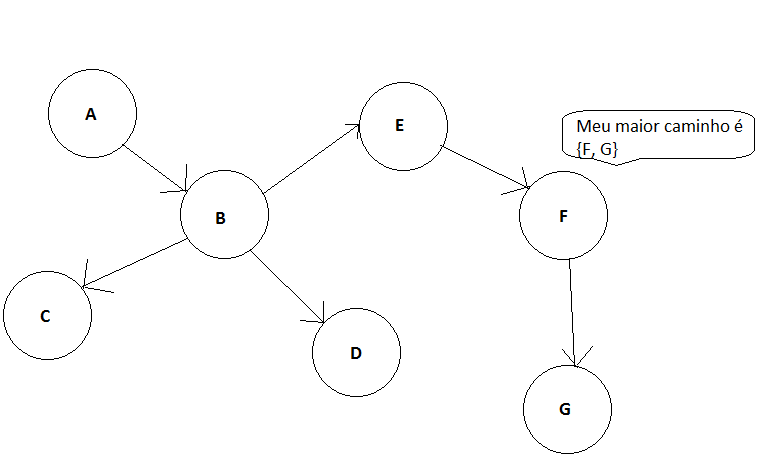
\includegraphics[width=100mm]{graphFr.png}
\caption{F respondendo à E}
\label{graphFr}
\end{figure}

\begin{figure}[H]
\centering
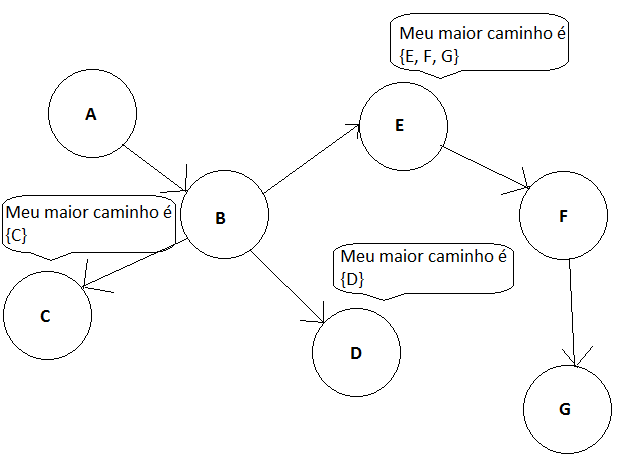
\includegraphics[width=100mm]{graphCrDrEr.png}
\caption{C, D e R respondendo à B}
\label{graphCrDrE}
\end{figure}

\begin{figure}[H]
\centering
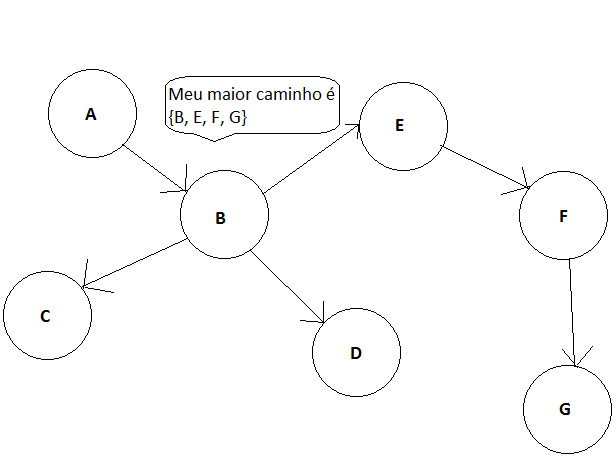
\includegraphics[width=100mm]{graphBr.png}
\caption{B respondendo à A}
\label{graphBr}
\end{figure}

\begin{figure}[H]
\centering
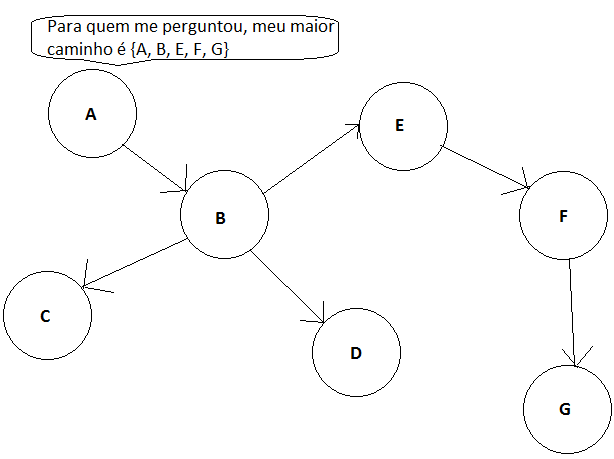
\includegraphics[width=100mm]{graphAr.png}
\caption{A respondendo à quem chamou}
\label{graphAr}
\end{figure}

Se esse método for chamado para todos os nodos de um grafo qualquer, e de todas
as respostas escolhermos a maior, teremos o maior caminho possível, ou no nosso
caso, a maior sequência de filmes. Essa é exatamente a idéia do nosso algoritmo.

Antes de mostrarmos como fica esse método em pseudo-código, há dois detalhes que
levamos em consideração na hora de implementar, e se não forem considerados, o
desempenho do algoritmo se torna péssimo. Vamos abordar cada um de uma forma bem
detalhada.

\subsection{Nodos fonte e nodos não-fonte}

Vamos definir os nodos em 2 tipos: Nodos fonte, e nodos não-fonte. Um nodo fonte
é um nodo que não tem nenhum outro apontando pra ele, um nodo não-fonte possui
nodos apontando para ele. Vamos olhar novamente o grafo usado anteriormente:

\begin{figure}[H]
\centering
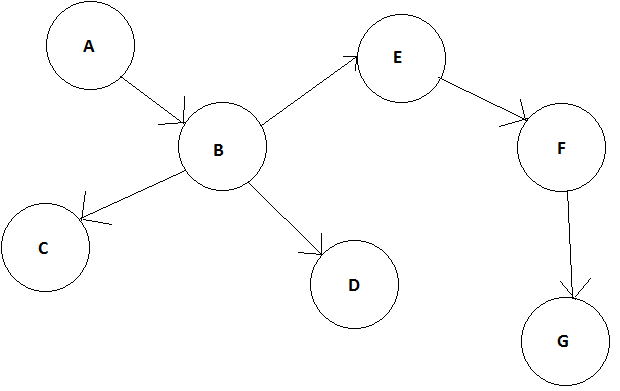
\includegraphics[width=100mm]{graph.png}
\caption{Exemplo 1}
\label{graphex}
\end{figure}

O nodo $A$ é um nodo fonte, já que não tem como chegar nele a partir de outro
nodo, nenhum nodo aponta para ele. Os demais são nodos não-fontes, já que algum
outro nodo aponta para eles. Por que isso é importante? Sempre que perguntarmos
para um nodo, chamarmos o método com ele de maior caminho, a resposta que ele
retorna é a maior resposta dos vizinhos. Seus vizinhos, com certeza, não são
fontes, ou seja, a maior resposta que tu recebe de um nodo não-fonte, não é o
maior caminho do grafo, pois para todo nodo não-fonte, existe um nodo que aponta
para ele e seria incluido no maior caminho.

Olhando para o grafo da figura~\ref{graphex}, se chamarmos o método para o nodo
$E$, a resposta vai ser $\{E, F, G\}$, mas o nodo $B$ aponta para $E$, se
chamarmos o método pra $B$, o retorno será $\{B, E, F, G\}$, mas o nodo $A$
aponta para $B$, se chamarmos o método para $A$, a resposta vai ser $\{A, B, E,
F, G\}$, como nenhum nodo aponta para $A$, é garantido que esse é o maior
caminho, já que nesse grafo só existe um nodo fonte.

Levando isso em consideração, o método para a achar a maior sequência de filmes,
só precisa ser chamado para os nodos fontes, pois eles garantem o maior caminho
entre todos os nodos não-fonte que são possíveis de chegar a partir dele.

\vspace{0.5cm}

Agora vamos analizar o segundo detalhe.

\subsection{Um nodo deve guardar o seu maior caminho}

Com tudo que foi explicado até agora, o rendimento do algoritmo continua sendo
péssimo. Do jeito que está, toda vez que se chega em um nodo, é necessário
descobrir seu maior caminho. Vamos imaginar a seguinte situação:

\begin{figure}[H]
\centering
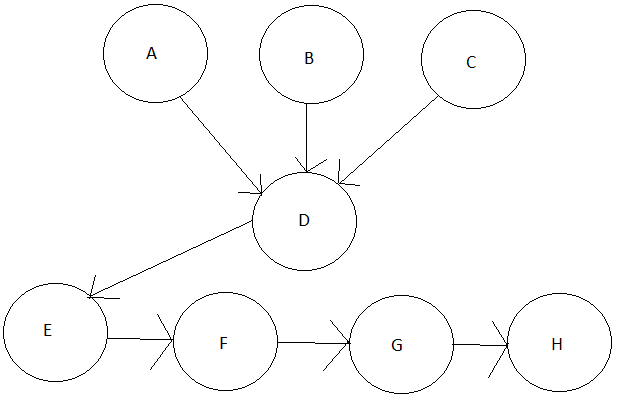
\includegraphics[width=100mm]{grafo.png}
\caption{Exemplo 2}
\label{grafo}
\end{figure}

$A$, $B$ e $C$ são nodos fonte, seguindo nosso algoritmo do jeito que está, o
método será chamado para esses três nodos. Esses nodos, vão chamar o método para
seus vizinhos, que no caso, é somente o nodo $D$. Seguindo por ordem alfabética,
quando $A$ pergunta para $D$ qual o seu maior caminho, o que acontece? $D$ não
sabe qual é seu maior caminho, ele vai perguntar para $E$, que pergunta para
$F$, que pergunta para $G$, que pergunta para $H$, e $H$ sabe responder já que
não tem vizinhos. A resposta vai voltando graças a recursão e $A$ descobre qual
é seu maior caminho. Agora é a vez do $B$ saber seu maior caminho, o que ele
faz? Pergunta para $D$ qual é o dele, e lá vai a recursão novamente até o nodo
$H$. Quando for a vez de $C$, o mesmo processo vai ocorrer, o nodo $D$ está
tendo que descobrir seu maior caminho três vezes! Não há necessidade de isso
acontecer, a resposta será sempre a mesma!

Isso é um problema péssimo, pois se mil nodos diferentes tiverem $D$ como
vizinho, ele vai ter que descobrir seu maior caminho mil vezes. Como vencer esse
problema? Uma vez que um nodo descubra seu maior caminho, ele guarda ela para
caso algum outro nodo perguntar, simples assim. A forma de guardar essa
informação pode ser de muitos jeitos, nós optamos por usar o tipo abstrato de
dado Lista, que vai guardar todos os nodos do maior caminho. Agora, voltando ao
exemplo anterior, se mil nodos diferentes tiverem $D$ como vizinho, ele descobre
apenas uma vez qual o seu maior caminho, e para todos os outros que perguntarem
ele já vai ter a resposta em mãos.

Esse é o ponto-chave desse algoritmo, se isso não for considerado, sua
velocidade de execução diminui de uma maneira absurda, já que o número de vezes
que um nodo teria que descobrir seu maior caminho, é o número de nodos que
possuem esse mesmo nodo como vizinho.

\subsection{Pseudo-Código}

Levando em consideração os dois detalhes mencionados anteriormente, a lógica de
implementação do nosso algoritmo foi essa:

\begin{lstlisting}

Lista numeroMaxFilmes() {
  Lista lista = nova lista vazia;
  para todo nodo u do grafo {
    se (u for um nodo fonte)
      Lista tmp = numeroMaxFilmes(u);
      se (tmp.tamanho > lista.tamanho)
        lista = tmp;
  }
  retorna lista;
}

\end{lstlisting}

Esse método vai ser chamado para todos os nodos fontes e tem como retorno o
maior caminho do grafo, que no nosso contexto representa o maior número possível
de filmes a ser assistido um após o outro.

\vspace{5.0cm}

\begin{lstlisting}

Lista numeroMaxFilmes(Node u) {
  Lista maior = nova lista vazia;
  se (u.getFilmes() == nulo) {          //u nao souber seu maior caminho
    para todos nodos v vizinhos de u {
      Lista aux = numeroMaxFilmes(v);
      se (maior.tamanho < aux.tamanho)
        maior = aux;
    }
    u.setFilmes(new ArrayList<Node>(maior));
  } senao {
    maior = u.getFilmes();
  }
  maior.add(0, u);                      //se adiciona na lista antes de retornar
  retorna maior;
}  

\end{lstlisting}

Esse é o método recursivo que descobre o maior caminho a partir de um nodo, que
vai ser chamado para cada nodo fonte do grafo.

\section{Resultados}

Quando nós nos demos conta do segundo detalhe, que dava para guardar o maior
caminho de um nodo em uma lista, o programa já estava sendo testado, o que se
tornou muito bom, pois até o caso de teste ex100, foi coletado o tempo de
execução sem a otimização.

\begin{table}[H]

\centering

\begin{tabular}{|c|c|c|c|c|c|}

\hline
Caso de teste & ex20 & ex40 & ex60 & ex80 & ex100 \\
\hline
Maior Sequência & Filme 3 & Filme 19 & Filme 18 & Filme 5 & Filme 99 \\
\cline{2-6}
& Filme 19 & Filme 8 & Filme 14 & Filme 19 & Filme 48\\
\cline{2-6}
& Filme 12 & Filme 25 & Filme 42 & Filme 8 & Filme 10\\
\cline{2-6}
& Filme 4 & Filme 24 & Filme 53 & Filme 65 & Filme 20\\
\cline{2-6}
& Filme 13 & Filme 2 & Filme 26 & Filme 33 & Filme 37\\
\cline{2-6}
& Filme 2 & Filme 32 & Filme 10 & Filme 30 & Filme 55\\
\cline{2-6}
& Filme 8 & Filme 34 & Filme 27 & Filme 52 & Filme 21\\
\cline{2-6}
& Filme 16 & Filme 4 & Filme 2 & Filme 22 & Filme 77\\
\cline{2-6}
& Filme 6 & Filme 10 & Filme 1 & Filme 24 & Filme 94\\
\cline{2-6}
& Filme 1 & Filme 3 & Filme 30 & Filme 20 & Filme 56\\
\cline{2-6}
& Filme 9 & Filme 12 & Filme 59 & Filme 12 & Filme 12\\
\cline{2-6}
& Filme 14 & Filme 22 & Filme 8 & Filme 18 & Filme 26\\
\cline{2-6}
& - & Filme 5 & Filme 44 & Filme 61 & Filme 82\\
\cline{2-6}
& - & - & Filme 17 & Filme 68 & Filme 2\\
\cline{2-6}
& - & - & Filme 45 & Filme 42 & Filme 54\\
\cline{2-6}
& - & - & Filme 13 & Filme 11 & Filme 65\\
\cline{2-6}
& - & - & Filme 52 & Filme 15 & Filme 16\\
\cline{2-6}
& - & - & - & Filme 23 & Filme 96\\
\cline{2-6}
& - & - & - & - & Filme 58\\
\cline{2-6}
& - & - & - & - & Filme 14\\
\cline{2-6}
& - & - & - & - & Filme 36\\
\cline{2-6}
& - & - & - & - & Filme 97\\
\cline{2-6}
& - & - & - & - & Filme 15\\
\hline
Tempo SO & 47ms & 505ms & 20049ms & 2181563ms & 41797664ms\\
\hline
Tempo & 1ms & 4ms & 9ms & 19ms & 17ms\\
\hline
Qtd Filmes & 12 & 13 & 17 & 18 & 23\\
\hline

\end{tabular}
\label{Tabela1}
\caption{Dados de ex20 - ex100}

\end{table}

Tempo SO - Tempo sem otimização, o nodo não armazena seu maior caminho. Dessa
maneira, só foi testado até o caso de teste ex100.

\begin{table}[H]

\centering

\begin{tabular}{|c|c|c|c|c|c|}

\hline
Caso de teste & ex120 & ex140 & ex160 & ex180 & ex200 \\
\hline
Maior Sequência & Filme 14 & Filme 68 & Filme 14 & Filme 35 & Filme 22 \\
\cline{2-6}
& Filme 28 & Filme 3 & Filme 6 &  Filme 37 & Filme 5 \\
\cline{2-6}
& Filme 4 & Filme 120 & Filme 23 & Filme 16 & Filme 137 \\
\cline{2-6}
& Filme 75 & Filme 33 & Filme 52 & Filme 167 & Filme 70 \\
\cline{2-6}
& Filme 109 & Filme 106 & Filme 43 & Filme 160 & Filme 66 \\
\cline{2-6}
& Filme 53 & Filme 93 & Filme 39 & Filme 109 & Filme 1 \\
\cline{2-6}
& Filme 48 & Filme 9 & Filme 128 & Filme 68 & Filme 20 \\
\cline{2-6}
& Filme 37 & Filme 51 & Filme 118 & Filme 103 & Filme 161 \\
\cline{2-6}
& Filme 87 & Filme 50 & Filme 67 & Filme 176 & Filme 49 \\
\cline{2-6}
& Filme 51 & Filme 82 & Filme 31 & Filme 17 & Filme 31 \\
\cline{2-6}
& Filme 71 & Filme 19 & Filme 7 & Filme 19 & Filme 93 \\
\cline{2-6}
& Filme 33 & Filme 4 & Filme 104 & Filme 53 & Filme 4 \\
\cline{2-6}
& Filme 5 & Filme 27 & Filme 156 & Filme 14 & Filme 44 \\
\cline{2-6}
& Filme 3 & Filme 28 & Filme 62 & Filme 67 & Filme 55 \\
\cline{2-6}
& Filme 63 & Filme 112 & Filme 1 & Filme 57 & Filme 77 \\
\cline{2-6}
& Filme 34 & Filme 59 & Filme 93 & Filme 30 & Filme 123 \\
\cline{2-6}
& Filme 8 & Filme 122 & Filme 140 & Filme 87 & Filme 120 \\
\cline{2-6}
& Filme 61 & Filme 11 & Filme 122 & Filme 105 & Filme 171 \\
\cline{2-6}
& Filme 1 & Filme 105 & Filme 19 & Filme 25 & Filme 40 \\
\cline{2-6}
& Filme 38 & Filme 39 & Filme 34 & Filme 180 & Filme 3 \\
\cline{2-6}
& Filme 42 & Filme 1 & Filme 3 & Filme 3 & Filme 7 \\
\cline{2-6}
& Filme 108 & Filme 52 & Filme 18 & Filme 73 & Filme 17 \\
\cline{2-6}
& Filme 16 & Filme 56 & Filme 15 & Filme 125 & Filme 50 \\
\cline{2-6}
& - & Filme 70 & - & Filme 29 & Filme 110 \\
\cline{2-6}
& - & Filme 79 & - & Filme 56 & Filme 94 \\
\cline{2-6}
& - & Filme 40 & - & Filme 21 & Filme 126 \\
\cline{2-6}
& - & Filme 80 & - & Filme 8 & Filme 101 \\
\cline{2-6}
& - & Filme 77 & - & Filme 40 & - \\
\cline{2-6}
& - & - & - & Filme 94 & - \\
\hline
Tempo & 2ms & 2ms & 3ms & 3ms & 3ms \\
\hline
Qtd Filmes & 23 & 28 & 23 & 29 & 27\\
\hline

\end{tabular}
\label{Tabela2}
\caption{Dados de ex120 - ex200}

\end{table}

Os algoritmos foram implementados em Java e rodaram em cima de um Intel(R)
Core(TM) i5-3210M CPU @ 2.50GHz 2.50GHz.

\section{Conclusões}

Sendo implementado de uma maneira correta, o algoritmo apresenta um desempenho
excelente, a resposta é praticamente imediata. Algo muito curioso, é que o tempo
de execução não aumenta junto com o número de nodos do grafo, por quê? Vamos
imaginar a seguinte situação: Um nodo $u$ com um grande número vizinhos, que por
sua vez possuem mais vizinhos e assim vai. Ao usarmos o algoritmo para esse
grafo, $u$ vai ter que esperar a resposta de todos os seus vizinhos, que vão ter
que esperar a resposta de seus vizinhos. Agora, se esse mesmo número de nodos
estiverem organizados na forma de uma lista, deixa de ser um grafo? Não, e se
chamarmos o método para $u$, a recursão só vai até o final da lista e volta, um
processo muito mais simples e rápido. A velocidade na hora da execução depende
muito mais do número de arestas.

Acreditamos ter desenvolvido uma solução eficiênte, eficaz, e simples de ser
compreendida. Apresentou resultados ótimos para todos os casos de teste,
demonstrando que mesmo sendo um problema relativamente complexo, devido ao
número de possibilidades, existe um jeito rápido de achar a solução.

\end{document}
